%%%%%%%%%%%%%%%%%%%%%%%%%%%%%%%%%%%%% BEGIN HEADERS %%%%%%%%%%%%%%%%%%%%%%%%%%%%%%%%%%%%%%%%%%%%%%%%%%%%%
\documentclass[11pt,conference]{IEEEtran}

\usepackage{longtable}
\usepackage{graphicx}
\usepackage[utf8]{inputenc}
\usepackage{fancyhdr}
\usepackage{float}
\usepackage[hidelinks]{hyperref}
\usepackage{listings}
\usepackage{color}
\usepackage{natbib}

% Your names in the header
\pagestyle{fancy}
\rhead{Enrico Tedeschi, Mike Murphy}
\lhead{INF-3200 Distributed Systems - Assignment 1}
\cfoot{\thepage}

% Used for including code in a stylized manner
\definecolor{codegreen}{rgb}{0,0.6,0}
\definecolor{codegray}{rgb}{0.5,0.5,0.5}
\definecolor{codepurple}{rgb}{0.58,0,0.82}
\definecolor{backcolour}{rgb}{0.95,0.95,0.92}
 

\lstdefinestyle{mystyle}{
    backgroundcolor=\color{backcolour},   
    commentstyle=\color{codegreen},
    keywordstyle=\color{magenta},
    numberstyle=\tiny\color{codegray},
    stringstyle=\color{codepurple},
    basicstyle=\footnotesize,
    breakatwhitespace=false,         
    breaklines=true,                 
    captionpos=b,                    
    keepspaces=true,                 
    numbers=left,                    
    numbersep=5pt,                  
    showspaces=false,                
    showstringspaces=false,
    showtabs=false,                  
    tabsize=2
}

\lstset{style=mystyle}

% The Title
\title{UiT INF-3200 Distributed Systems - Project 1\\Fall 2015}

% Your name and email
\author{Enrico Tedeschi\\ete011@post.uit.no
    \and Mike Murphy\\mmu019@post.uit.no}


%%%%%%%%%%%%%%%%%%%%%%%%%%%%%%%%%%%%% END HEADERS %%%%%%%%%%%%%%%%%%%%%%%%%%%%%%%%%%%%%%%%%%%%%%%%%%%%%

\begin{document}

% Create the title and everything
\maketitle


\section{Introduction}

Our task was to implement a simple distributed key-value store.

The general idea is to have a number of back-end nodes that store data, and a
front-end node that forwards requests into the back-end group. The front-end
should be able to contact any storage node and get the same results.


\subsection{Requirements}

Our data store \ldots

\begin{itemize}
\item must incorporate multiple storage nodes.
\item must work without any node having complete knowledge of the others.
\item must work no matter which storage node the front-end contacts. For
    testing, the front-end should contact random nodes.
\item does not need to support dynamic adding and removal of storage nodes.
\item does not need to persist data between runs.
\end{itemize}


\section{Technical Background}



\begin{itemize} 
\item[--] Distributed systems concept
\item[--] Basic programming approach
\item[--] Knowledge of Python language
\item[--] Notion of design pattern principles
\item[--] Theory about software engineering
\item[--] Knowledge of git to manage the software versions
\item[--] Notion of Chord architecture
\item[--] Basic approach to Linux command line
\end{itemize}


\section{Design}

We arranged our key space along one dimension in a ring, following the lead of
Chord\cite{chord}. Regions of the key space are assigned to each node. Each node
is aware of the range of key space that it is responsible and the next node in
the ring (Fig \ref{fig:design}). If a node receives a request to store or retrieve a key that is not in
its range, it will forward the request to the next node.

Though our design was inspired by Chord, we did not implement Chord's finger
table optimization, for lack of time.

Because all nodes are known ahead of time, with no joining or leaving, we could
divide the key space evenly between each node.

For forwarding requests to successor nodes, we used a simple synchronous
strategy: the node's request-handler thread will block while it contacts the
next node. This was the easiest to implement, but it is wasteful of resources.

\begin{figure}[h!]
  \centering
    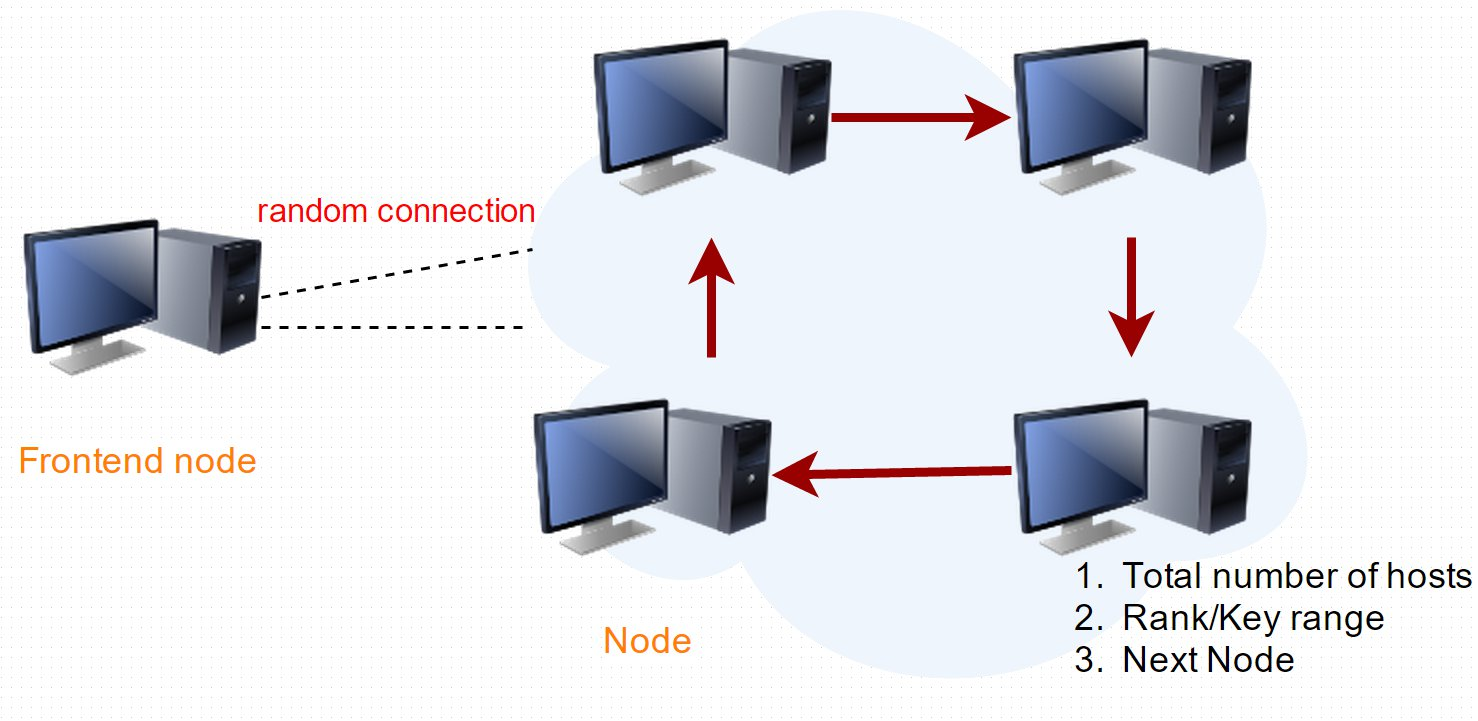
\includegraphics[width=0.5\textwidth]{design}
    \caption{Design of the implemented Network}
    \label{fig:design}
\end{figure}


\section{Implementation}


\subsection{Languages and Code}

Our solution is implemented in a mix of Python and shell script, Python for the
actual node and front-end programs, and a shell script to start up and shut down
nodes via SSH.

We started with skeleton code by our teaching assistants, Einar Holsbø Jakobsen
and Magnus Stenhaug, which included the front-end code and the startup/shutdown
shell script. Their front-end also included an automated test routine that
rapidly inserted and retrieved random key-value pairs.

We wrote the actual storage node code, and we also made a few enhancements to
the startup shell script. We modified the startup script to pick a randomized
set of computers from the cluster for each test run. This randomization was to
prevent our test runs from occupying too much time on any particular machines.


\subsection{Network Protocol}

The backend nodes accept and retrieve data through a simple HTTP API. HTTP's PUT
and GET operations are a natural fit for a key-value store, as their semantics
specify storing and retrieving documents (value) at a given URL path (key).
Jakobsen and Stenhaug chose this protocol for their starter front-end node and
we expanded it to the storage nodes.


\subsection{Persistence}

The purpose of this exercise was to investigate the challenges of distributed
data storage, not storage itself. Therefore, there was no requirement to
actually persist stored data between runs. So, for simplicity, we did not
implement any kind of data persistence. Data is simply stored in memory and the
store starts empty on each test run.

\subsection{Frontend}

The \textit{Frontend Node} (Fig \ref{fig:frontend}) has been modified considering an approach more close to the reality. It takes as input a list of nodes and a random one is chosen to get the requests.
In that way a distributed transparency is provided since it doesn't matter from which node the frontend will connect because it will get the result anyway by reason of the nodes are communicating each others.

\begin{figure}[h!]
  \centering
    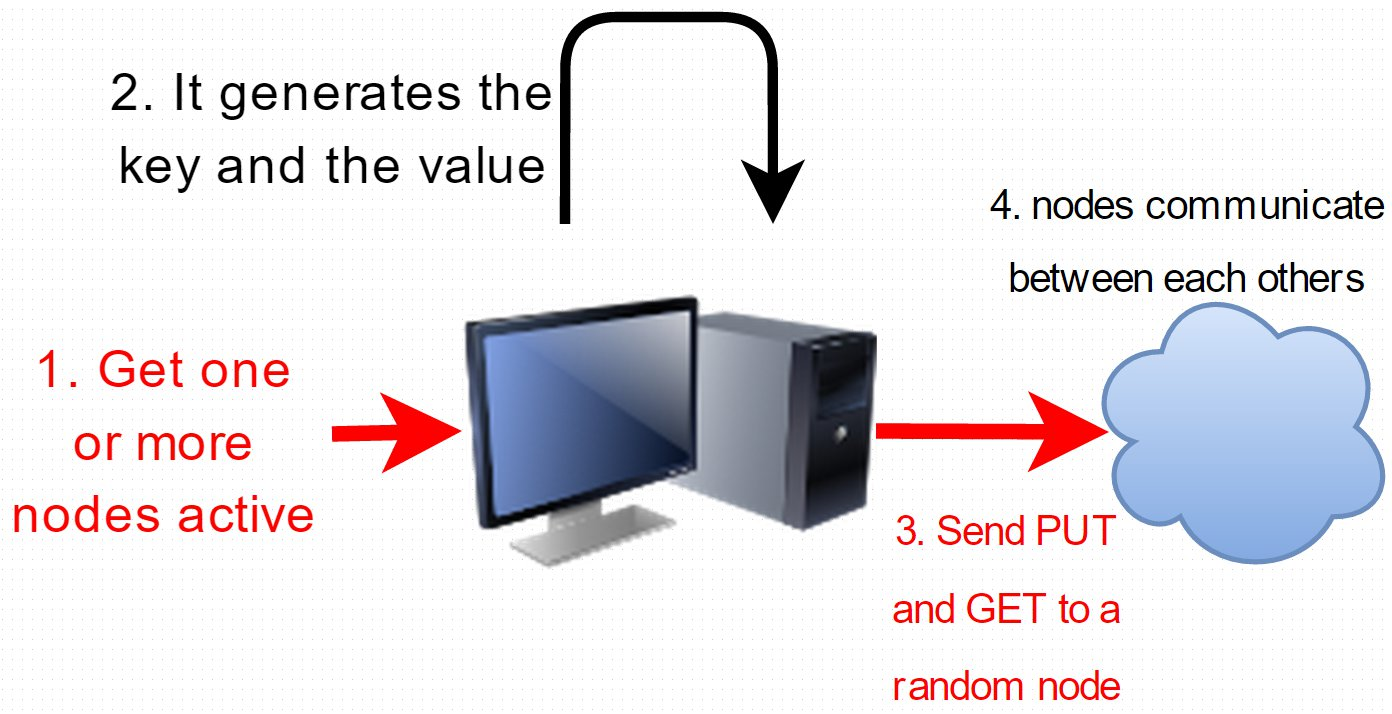
\includegraphics[width=0.5\textwidth]{frontend}
    \caption{Implementation of the Frontend node}
    \label{fig:frontend}
\end{figure}

\subsection{Node}

Each node (Fig \ref{fig:node}) has a really simple workflow. It starts running and waits for a request, which could be GET or PUT from the \textit{Frontend} node. A class \textit{node\_request} has been implemented to keep the \textit{http} logic separates from the node logic, having in that way an easier approach to the testing part and avoiding to have a fat class, respecting a principle of the design pattern.
When the node gets a request it checks if is supposed to be for him, if yes then the request will be executed and the response is sent to the Frontend, otherwise the Node forward the request through the class \textit{node\_request} to the next node.
Each node knows exactly which range of key to store thank to an md5 hash. The md5 function is in the node class and for each key an hash value is provided.
To be sure that the node is working on the key that is supposed to be for him, this method was implemented:

\begin{lstlisting}
 def responsible_for_key(key):
        key_hash = node_hash(key)
        rank_resp = key_hash % self.node_count
        return rank_responsible == self.rank
\end{lstlisting}
Where the function \textit{node\_hash(key)} takes care of converting a given key into a md5 hashed value and \textit{rank\_resp} is the node which is responsible to execute the requested operation, obtained using the module function on the total number of nodes.
\newline
A function \textit{hash()} exists already in python libraries but we used the md5 cryptographic hashing for problems related to security for the possible future implementations.

\begin{figure}[h!]
  \centering
    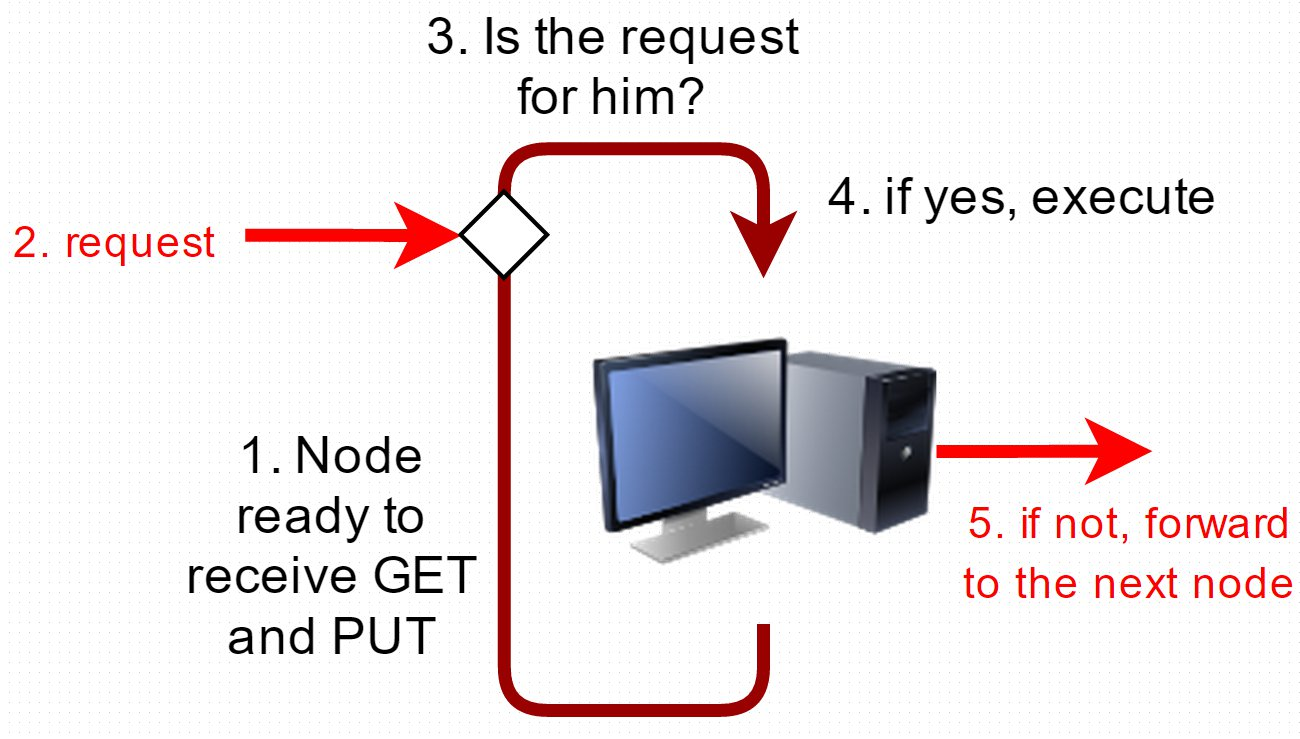
\includegraphics[width=0.5\textwidth]{node}
    \caption{Implementation of the Node}
    \label{fig:node}
\end{figure}


\subsection{Environment}

Our code was written to run on the Rocks Cluster distribution\cite{rocks}, and
makes some assumptions about that environment. We rely on the cluster's shared
filesystem for distributing program code to servers. And we rely on easy SSH
access between machines in the cluster to start and shutdown nodes.


\section{Discussion}

Our design decisions favored simplicity over performance. The simple ring
structure was easy to implement, but requests may need to be forwarded along
several nodes in the ring before finding the correct key. The number of hops is
linear with the number of nodes, $O(n)$. Chord's finger-table
optimization\cite{chord} finds nodes in $O(\log_2 n)$ hops. We had hoped to
implement the same strategy in our project but we ran out of time.

The simple synchronous request forwarding strategy is also a potential
bottleneck. It leaves a thread idle on each node involved in each request,
waiting until the right key is found before returning it back through all of the
nodes that were involved. We suspect that, as the number nodes grows or request
frequency increases, this holding of resources will choke the system. The
advantage of this approach is its simplicity. The request and response protocol
is identical between client and front-end, front-end and storage node, and
between storage nodes themselves. The storage nodes also use the same logic to
handle requests whether the request comes from the front-end or another node in
the chain.

Asynchronous message-passing would allow intermediate nodes in a search to free
resources. The first node could block, and then send a message to the next node.
If this message included a return address to the first node, then the other
nodes in the ring could pass it along without leaving connections open or
blocking. Finally, the node that has the key could send the value to original
node. When that original node received its answer, it could unblock and send the
response to the front-end. Such a strategy should be more efficient, but would
require different message formats for requests and answers, and nodes would need
logic to receive answer messages and match them to waiting threads to send
responses. We suspect that the finger tables would give a much larger
performance boost. Not only that, but with $O(\log_2 n)$ searching, only a few
nodes would be involved in each search, and the overhead from waiting
synchronously on just a few nodes might be acceptable.


\section{Evaluation}

% TODO: time actual implementation


\section{Conclusion}

% TODO: Conclusion


\section{CITATION PLACEHOLDER}

% TODO: Remove section
This text is only here to hang some citations before they're used in the real
text.
\cite{linuxjournal_dht}
\cite{chord}
\cite{parallel}
\cite{Balakrishnan:2003:LUD:606272.606299}


\bibliographystyle{plain}
\bibliography{report}


\end{document}
